\documentclass[a4paper,11pt]{article}
\usepackage[english]{babel}
\usepackage[utf8]{inputenc}
\usepackage{geometry}

\usepackage{booktabs}  
\usepackage{graphicx} 
\usepackage{listings}
\usepackage{booktabs,adjustbox}
\usepackage{amsmath}
\usepackage[tableposition=top]{caption}


\usepackage{pdflscape}
\lstset{%
backgroundcolor=\color{black},
basicstyle=\ttfamily,
numbers=left,numberstyle=\scriptsize
}

\usepackage{hyperref}
\hypersetup{
    colorlinks=true,
    linkcolor=blue,
    filecolor=magenta,      
    urlcolor=blue,
    citecolor=black
}


\usepackage{natbib}

\usepackage[wby]{callouts}

\graphicspath{ {./report/visualisations/} }

\title{SCAN*PRO: Understanding the effectiveness of price, display and promotional activity for competing brands of beer  \\
\addlinespace
\large Retail Marketing Analytics - Individual Report}
\author{Julian West | CID 01623906}


\begin{document}

\maketitle
\begin{abstract}
In this analysis, the SCAN*PRO model is applied to understand the effect of promotional activity on the unit sales of three competing brands of beer sold by a supermarket store. This information can be used by the store manager to more effectively utilise promotions to increase unit sales for each brand of beer. Three separate SCAN*PRO models were created, one for each brand, to estimate the own and cross brand elasticities for price, display and feature promotional activity whilst also incorporating the effect of seasonality on sales. Beer sales for all three brands were highly seasonal with unit sales increased up to 45\% in the summer months. Feature promotions were found to be more effective than display promotions, however, ....

\end{abstract} \hspace{50pt}

\newpage
\tableofcontents
\newpage

\section{Introduction}
Retailers are interested in understanding the impact that promotional activity has on product sales. This information can aid short term demand forecasting and help optimise the allocation of limited promotion resources. The SCAN*PRO model \citep{wittink_estimation_1988} is a popular method for quantifying the interaction effects between various promotional activities such as price reductions, display promotions and feature promotions, allowing store mangers to understand the effectiveness of promotional campaigns for different products \citep{andrews_estimating_2008, srinivasan_promotions_2004}. 

In this analysis, the SCAN*PRO model was be used to understand the effects of promotional activity on the sales of three competing brands of beer for a Chicago based supermarket store, Dominick's. The insights gained from the model were used to make recommendations to the store manager on how to tailor promotional activity for each brand of beer to effectively use their promotional activity resources.

\subsection{Business Objective \& Research Question}
The following business objective and corresponding research questions were evaluated in the analysis:
\newline
\newline
\textbf{Business Objective}: What is the most effective form of promotion to boost unit sales of each beer brand?
\begin{itemize}
        \item Which types of promotion are more effective for each beer brand: price reduction, display or feature promotion?
        \item Are promotions equally effective for each brand of beer?
        \item How does promotional activity of each brand interact with sales of other beer brands?
\end{itemize}
\newline
\newline

This analysis will look at promotional activity from the perspective of the store manager making decisions on retail pricing and on how many stock units should be promoted in a given week. The research questions answered in the analysis aim to inform how the store manager can make best use of limited promotional resources to sell more units of beer. 

\subsection{Assumptions}

The main assumptions of the analysis are as follows:
\begin{itemize}
    \item There is a finite amount of promotional resource, therefore there is a benefit to optimising the promotional activity for brands which have the best response to certain types of promotion.
    \item The manager has full control over setting the level of feature, display and price promotional activity. For example, there are no contractual obligations with brand suppliers which guarantees a certain level of promotion.
\end{itemize}


\subsection{About SCAN*PRO}

SCAN*PRO is a store-level model which is able to quantify the effect of price changes and promotional activities on the unit sales of products for retailers. The model is a multiplicative model which includes own and cross brands elasticities for price, feature and display advertising. Seasonality and a random error term are also included in the model. The SCAN*PRO model is shown in equation \ref{eqn:scanpro}  \citep{leeflang_how_2002}:
\begin{equation}
\label{eqn:scanpro}
    q_{kjt} = \Bigg[\prod_{r=1}^n\Bigg(\frac{p_{krt}}{\bar{p}_{kr}}\Bigg)^{\beta rj}\prod_{t=1}^{T}\gamma_{lrj}^{D_{lkrt}}\Bigg]\Bigg[\prod_{t=1}^{T}\delta_{jt}^{X_{t}}\Bigg]\Bigg[\prod_{k=1}^{K}\lambda_{kj}^{Z_{k}}\Bigg]e^{u_{kjt}} 
\end{equation}

For $k = 1, ...., K; t=1,....T$
\newline
\newline
Where:
\begin{itemize}
    \item $q_{kjt}$: unit sales for brand $j$ in store $k$ in week $t$
    \item $p_{krt}$: unit price for brand $r$ in store $k$ in week $t$
    \item $D_{1krt}$: indicator variable for display advertising: 1 if brand $r$ is displayed 0 if not
    \item $D_{2krt}$: indicator variable for feature advertising: 1 if brand $r$ is featured 0 if not
    \item $X_t$: indicator variable (for seasonal effects)
    \item $Z_k$: indicator variable for store $k$
    \item $e$: error term for unobserved or missing variables from the model
\end{itemize}

The parameters $\beta_{rj}$, $\gamma_{lrj}$, $\delta_{jt}$ and $\lambda_{kj}$ are to be estimated. These parameters can be estimated using non-linear optimisation techniques, however, this can be computationally expensive, highly sensitive to model inputs and has no guarantee of reaching a global minimum. Therefore, it is advantageous to take the log transformation of equation \ref{eqn:scanpro} to make the model additive which can be solved using simple linear estimation techniques such as OLS. 

The additive model to be estimated thus becomes:
\begin{equation}
\label{eqn:scanprolog}
    ln(q_{kjt}) = \sum_{r=1}^n{\beta _{rj}ln\Bigg(\frac{p_{krt}}{\bar{p}_{kr}}\Bigg)+ \sum_{r=1}^n\sum_{l=1}^{2}{ln(\gamma_{lrj}){D_{lkrt}}}} + \sum_{t=1}^T{ln(\delta_{jt})X_t} + \sum_{k=1}^K{ln(\lambda_{kj})Z_k} + e_{kjt}
\end{equation}

The model parameters from equation \ref{eqn:scanprolog} can then be converted back into the multiplicative form in equation \ref{eqn:scanpro} to estimate unit sales for the week.


\subsection{Software Used}

All analysis was conducted using \href{https://www.python.org/}{Python (programming language)}. Details of code and packages used are included in the supplementary information.


\section{Data}
\subsection{Description}
The dataset used for the analysis consists of scanner records for beer category products from a grocery store, Dominick's Finer Foods store (Dominick's). The original source of the dataset was  \href{https://www.chicagobooth.edu/research/kilts/datasets/dominicks}{Chicago Booth Kilts Center for Marketing} and a description of the raw dataset is included in \citet{srinivasan_promotions_2004}. However, the dataset used for this analysis was an adapted dataset shared by the Imperial College Retail Marketing Analytics teaching team via Slack (March 19th - \emph{beer\_data\_chicago\_Dominicks.xlsx}).

The data covers 227 weeks (4 years 5 months) of sales for three brands of beer between 1989 and 1993. The raw data contains the following attributes for each brand:

\begin{table}[htb]
 \centering
 \caption{Raw dataset features}\label{tab:data_features}
 \begin{tabular}{cccc}
 \toprule
  Variable Name & Description \\
  \midrule
  \texttt{SALESBRAND*}& the average sales (\$) for brand * \\
  \texttt{PRICEBRAND*}	& the retail price (\$) for brand * \\
  \texttt{display\_brand*}	& the percentage of SKUs{$\dagger$} on display for brand * \\
  \texttt{FEATUREBRAND*}	& the percentage of SKUs featured in the store for brand * \\
  \texttt{RETAILERMARGINBRAND*} & the average retailer margin (\%) for brand * \\
  \texttt{WHOLESALEPRICEBRAND*} & the average wholesale price (\$) for brand * \\
  \bottomrule
  \multicolumn{2}{c}{$*$ Brand 1,2 or 3, $\dagger$ Stock keeping units}
 \end{tabular}
\end{table}

The display and feature attributes are expressed as the percentage of stock keeping units (SKUs) which were promoted by the store in a given week. It is not clear from the literature \citep{srinivasan_promotions_2004} what 'display' and 'feature' promotions specifically involved at the store so it is assumed that for a display promotion the product was displayed prominently in the store and for a feature promotion the product was 'on offer'. 

The raw data did not contain a \textit{unit sales} variable which is the desired target variable for the SCAN*PRO model. Therefore, a unit sales variable, \textit{UNITSBRAND*}, was created for each brand by dividing the sales of the brand by its average retail price for each week.

The retailer margin is not a factor in the SCAN*PRO model described in equation \ref{eqn:scanpro} and was therefore not considered in the model estimation.

The wholesale price is not directly used in the SCAN*PRO model as the retail price is used instead. However, retail prices can be subject issues with endogeneity as they may be set by the store manager in response to how well the the product is selling, and therefore may not completely independent of the target variable, unit sales. The wholesale price can be a useful alternative to retail price as an instrument variable if endogenity exists and was kept in the dataset for further investigation.



\subsection{Assumptions}
The data observations are given with weekly interval and it is assumed that the display and feature promotions lasted for the entire week of the observation.

The start date for the data observations was not explicit in the literature \citep{srinivasan_promotions_2004}. It was assumed that the data observations started in the first week of June 1989 (4th June 1989) which is consistent with the seasonality exhibited in figure \ref{fig:seasonal-plots}.

\subsection{Exploratory Analysis}


\begin{figure}
  \centering
  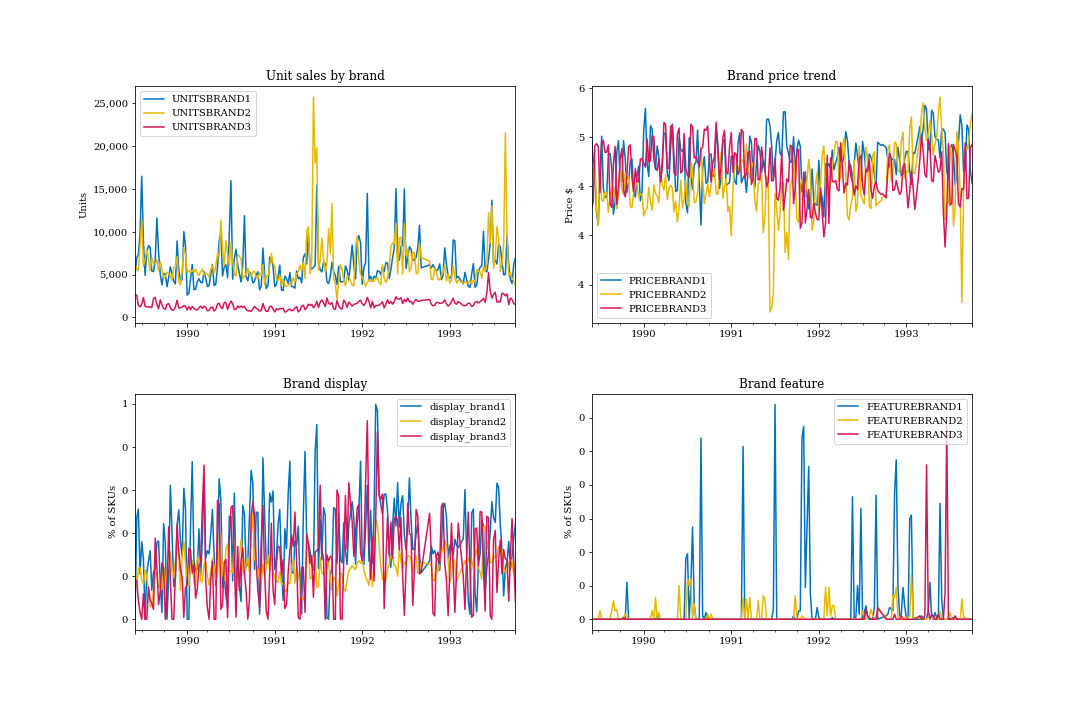
\includegraphics[scale=0.38]{eda_plots}
  \caption{Unit sales, price, display and feature data for each brand}\label{fig:eda-plots}
\end{figure}

The unit sales, prices, display and feature variables for each brand are shown in figure \ref{fig:eda-plots}. 

Brands 1 and 2 are the most popular with similar weekly unit sales but they also exhibit a greatest variation in unit sales from week to week. Whereas brand 3 has a much more consistent but lower sales volume. It appears most of the variation in unit sales is driven by seasonal factors.

The retail price of each brand is similar and hovers between approximately \$4 and \$5 throughout the time period. 

Each brand appears to have a certain percentage of stock keeping units 'on display' in almost every week. There is a very high variation in the percentage of SKUs from week to week ranging from 0\% to 50\%, with brand 1 having the highest average percentage of SKUs on display each week (14\%).

The 'feature' promotional activity appears to happen less frequently and used more sparingly than the 'display' promotions. Most weeks typically have no brands or just one brand featured. Brand 1 was featured the most and tended to have a greater percentage of SKUs featured in the week compared to when other brands were featured. Brand 2 was featured more consistently than the other brands albeit with a smaller percentage of SKUs. Brand 3 was only featured towards the end of the time period of observations. 

The SCAN*PRO model is also sensitive to seasonal effects in the unit sales. Figure \ref{fig:seasonal-plots} shows the seasonal component of the unit sales for each brand of beer. There are clear and significant seasonal trends in the data for all brands, with unit sales peaking in the summer months (May-August) as well as smaller peaks across the Christmas holiday period.


\begin{figure}
  \centering
  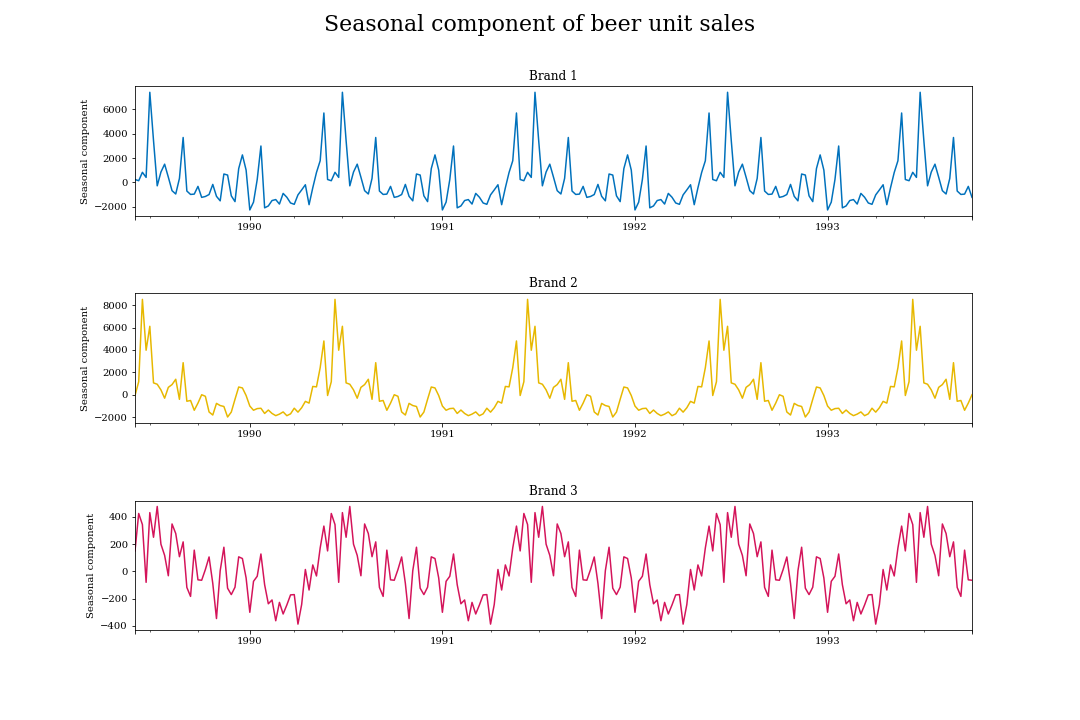
\includegraphics[scale=0.38]{seasonal_plots}
  \caption{Seasonal component of unit sales for each brand unit sales}\label{fig:seasonal-plots}
\end{figure}


\section{Model Estimation}
\subsection{Methodology}

\subsubsection{Data Preparation}
In order for the model to be estimated using linear methodologies (equation \ref{eqn:scanprolog}), the \textit{UNITSBRAND*}, \textit{PRICEBRAND*} and \textit{display\_brand*} variables were log transformed. Due to the presence of a small number of zero values in the \textit{display\_brand*} variables, a $log(x+1)$ transformation \citep{wooldridge_multiple_2016} was used to avoid \textit{-inf} values after the transformation.

The \textit{FEATUREBRAND*} variable could not be log transformed in this manner as the majority of values were zero for each brand (figure \ref{fig:eda-plots}) which would make interpretation of the coefficients less meaningful. Therefore the \textit{FEATUREBRAND*} variable was encoded as a new binary variable, \textit{binary\_FEATUREBRAND*}, which was labelled as 1 if the percentage of SKUs was greater than 0.02 and 0 otherwise. Even though the percentage of SKUs featured was not the same for each brand, the binary variable still preserved important information about the effects of feature promotions on unit sales.

Finally, eleven dummy variables ($k-1$) were created for each month of the year to encode the seasonality observed in figure \ref{fig:seasonal-plots}.


\subsubsection{Model Estimation \& Validation}
A separate model was created for each of the three competing brands of beer. The log unit sales (\textit{log\_UNITSBRAND*}) for each brand were estimated using a regression model with the \textit{log\_PRICEBRAND*}, \textit{log\_display\_brand*}, \textit{binary\_FEATUREBRAND*} and seasonal dummy variables as inputs (see \textit{notebooks/01\_regression\_modelling.ipynb} in the supplementary information). \footnote{Alternative combinations of model inputs were also investigated, however, these were deemed to be less accurate and were not selected for further investigation (see \textit{02\_alternative\_models.ipynb} in the supplementary information for analysis)}

To validate the models, 80\% of the data was randomly sampled for model estimation (training) with 20\% reserved for validating the accuracy of the model on unseen data. Once the model had been validated and the linear regression assumptions checked, the model was re-estimated using the full dataset to obtain the final model coefficients which could be used for interpretation.

Table \ref{tab:val-results} shows the $R^2$ of the SCAN*PRO model for each brand model trained on 80\% of the available data. All three models gave reasonably good $R^2$ values with the models explaining approximately 80\% of the variation in the data. The root mean squared error (RMSE) of the models on the unseen test data was approximately 0.17 for each model (equivalent to an average prediction error of $\pm 2\%$). The $R^2$ and RMSE for each model are consistent which suggests that the model is generalisable with good performance for all three brands.


\begin{table}
\centering
\caption{$R^2$ for models trained on 80\% of data and RMSE of model on unseen test data}\label{tab:val-results}
\begin{tabular}{lrr}
\toprule
Model &        $R^2$ &      RMSE \\
\midrule
Brand 1 &  0.792233 &  0.165940 \\
Brand 2 &  0.812804 &  0.172020 \\
Brand 3 &  0.813989 &  0.177375 \\
\bottomrule
\end{tabular}
\end{table}


\subsection{Results}
The final model coefficients for brand 1, 2 and 3 estimated using all available observations are reported in tables \ref{tab:brand1}, \ref{tab:brand2} and \ref{tab:brand3} respectively.

\newpage
\begin{center}
\begin{table}
\caption{Brand 1: SCAN*PRO coefficients}\label{tab:brand1}
\begin{tabular}{lclc}

\toprule
\textbf{Dep. Variable:}        & log\_UNITSBRAND1 & \textbf{  R-squared:         } &     0.777   \\
\textbf{Model:}                &       OLS        & \textbf{  Adj. R-squared:    } &     0.756   \\
\textbf{Method:}               &  Least Squares   & \textbf{  F-statistic:       } &     35.96   \\
\textbf{Date:}                 & Sat, 11 Apr 2020 & \textbf{  Prob (F-statistic):} &  3.77e-56   \\
\textbf{Time:}                 &     16:22:19     & \textbf{  Log-Likelihood:    } &    94.246   \\
\textbf{No. Observations:}     &         227      & \textbf{  AIC:               } &    -146.5   \\
\textbf{Df Residuals:}         &         206      & \textbf{  BIC:               } &    -74.57   \\
\textbf{Df Model:}             &          20      & \textbf{                     } &             \\
\bottomrule
\end{tabular}
\end{table}
\begin{tabular}{lcccccc}
                               & \textbf{coef} & \textbf{std err} & \textbf{t} & \textbf{P$> |$t$|$} & \textbf{[0.025} & \textbf{0.975]}  \\
\midrule
\textbf{const}                 &      18.8007  &        1.033     &    18.206  &         0.000        &       16.765    &       20.837     \\
\textbf{log\_PRICEBRAND1}      &      -4.8740  &        0.369     &   -13.209  &         0.000        &       -5.601    &       -4.146     \\
\textbf{log\_PRICEBRAND2}      &       0.3262  &        0.205     &     1.589  &         0.114        &       -0.079    &        0.731     \\
\textbf{log\_PRICEBRAND3}      &      -1.4018  &        0.362     &    -3.873  &         0.000        &       -2.115    &       -0.688     \\
\textbf{log\_display\_brand1}  &       0.6736  &        0.199     &     3.390  &         0.001        &        0.282    &        1.065     \\
\textbf{log\_display\_brand2}  &       0.7605  &        0.414     &     1.837  &         0.068        &       -0.056    &        1.577     \\
\textbf{log\_display\_brand3}  &      -0.3266  &        0.215     &    -1.521  &         0.130        &       -0.750    &        0.097     \\
\textbf{binary\_FEATUREBRAND1} &       0.0939  &        0.040     &     2.376  &         0.018        &        0.016    &        0.172     \\
\textbf{binary\_FEATUREBRAND2} &       0.0075  &        0.042     &     0.179  &         0.858        &       -0.075    &        0.090     \\
\textbf{binary\_FEATUREBRAND3} &       0.0148  &        0.107     &     0.138  &         0.890        &       -0.196    &        0.225     \\
\textbf{August}                &       0.2292  &        0.057     &     4.019  &         0.000        &        0.117    &        0.342     \\
\textbf{December}              &      -0.0772  &        0.061     &    -1.266  &         0.207        &       -0.198    &        0.043     \\
\textbf{February}              &      -0.1557  &        0.059     &    -2.625  &         0.009        &       -0.273    &       -0.039     \\
\textbf{January}               &      -0.0700  &        0.060     &    -1.174  &         0.242        &       -0.188    &        0.048     \\
\textbf{July}                  &       0.2674  &        0.056     &     4.737  &         0.000        &        0.156    &        0.379     \\
\textbf{June}                  &       0.3694  &        0.059     &     6.304  &         0.000        &        0.254    &        0.485     \\
\textbf{March}                 &      -0.1076  &        0.060     &    -1.796  &         0.074        &       -0.226    &        0.011     \\
\textbf{May}                   &       0.3299  &        0.058     &     5.658  &         0.000        &        0.215    &        0.445     \\
\textbf{November}              &      -0.0992  &        0.061     &    -1.633  &         0.104        &       -0.219    &        0.021     \\
\textbf{October}               &      -0.0726  &        0.058     &    -1.244  &         0.215        &       -0.188    &        0.042     \\
\textbf{September}             &       0.0766  &        0.055     &     1.383  &         0.168        &       -0.033    &        0.186     \\
\bottomrule
\end{tabular}
\begin{tabular}{lclc}
\textbf{Omnibus:}       & 11.282 & \textbf{  Durbin-Watson:     } &    1.446  \\
\textbf{Prob(Omnibus):} &  0.004 & \textbf{  Jarque-Bera (JB):  } &   11.511  \\
\textbf{Skew:}          &  0.520 & \textbf{  Prob(JB):          } &  0.00317  \\
\textbf{Kurtosis:}      &  3.366 & \textbf{  Cond. No.          } &     317.  \\
\bottomrule
\end{tabular}
\end{center}
\newpage

% BRAND 2 REGRESSION RESULTS
\begin{center}
\begin{table}
\caption{Brand 2: SCAN*PRO coefficients}\label{tab:brand2}
\begin{tabular}{lclc}
\toprule
\textbf{Dep. Variable:}        & log\_UNITSBRAND2 & \textbf{  R-squared:         } &     0.805   \\
\textbf{Model:}                &       OLS        & \textbf{  Adj. R-squared:    } &     0.786   \\
\textbf{Method:}               &  Least Squares   & \textbf{  F-statistic:       } &     42.52   \\
\textbf{Date:}                 & Sat, 11 Apr 2020 & \textbf{  Prob (F-statistic):} &  6.01e-62   \\
\textbf{Time:}                 &     16:36:52     & \textbf{  Log-Likelihood:    } &    111.22   \\
\textbf{No. Observations:}     &         227      & \textbf{  AIC:               } &    -180.4   \\
\textbf{Df Residuals:}         &         206      & \textbf{  BIC:               } &    -108.5   \\
\textbf{Df Model:}             &          20      & \textbf{                     } &             \\
\bottomrule
\end{tabular}
\end{table}
\begin{tabular}{lcccccc}
                               & \textbf{coef} & \textbf{std err} & \textbf{t} & \textbf{P$> |$t$|$} & \textbf{[0.025} & \textbf{0.975]}  \\
\midrule
\textbf{const}                 &      16.6887  &        0.958     &    17.416  &         0.000        &       14.799    &       18.578     \\
\textbf{log\_PRICEBRAND1}      &      -0.5023  &        0.342     &    -1.467  &         0.144        &       -1.177    &        0.173     \\
\textbf{log\_PRICEBRAND2}      &      -3.6822  &        0.190     &   -19.329  &         0.000        &       -4.058    &       -3.307     \\
\textbf{log\_PRICEBRAND3}      &      -0.6435  &        0.336     &    -1.916  &         0.057        &       -1.306    &        0.019     \\
\textbf{log\_display\_brand1}  &      -0.1127  &        0.184     &    -0.611  &         0.542        &       -0.476    &        0.251     \\
\textbf{log\_display\_brand2}  &       2.5825  &        0.384     &     6.724  &         0.000        &        1.825    &        3.340     \\
\textbf{log\_display\_brand3}  &      -0.3336  &        0.199     &    -1.675  &         0.095        &       -0.726    &        0.059     \\
\textbf{binary\_FEATUREBRAND1} &       0.0152  &        0.037     &     0.414  &         0.679        &       -0.057    &        0.087     \\
\textbf{binary\_FEATUREBRAND2} &       0.0325  &        0.039     &     0.841  &         0.401        &       -0.044    &        0.109     \\
\textbf{binary\_FEATUREBRAND3} &       0.0320  &        0.099     &     0.323  &         0.747        &       -0.163    &        0.227     \\
\textbf{August}                &       0.1409  &        0.053     &     2.662  &         0.008        &        0.037    &        0.245     \\
\textbf{December}              &      -0.0739  &        0.057     &    -1.306  &         0.193        &       -0.186    &        0.038     \\
\textbf{February}              &      -0.1645  &        0.055     &    -2.989  &         0.003        &       -0.273    &       -0.056     \\
\textbf{January}               &      -0.1237  &        0.055     &    -2.235  &         0.027        &       -0.233    &       -0.015     \\
\textbf{July}                  &       0.1566  &        0.052     &     2.989  &         0.003        &        0.053    &        0.260     \\
\textbf{June}                  &       0.2464  &        0.054     &     4.531  &         0.000        &        0.139    &        0.354     \\
\textbf{March}                 &      -0.0576  &        0.056     &    -1.035  &         0.302        &       -0.167    &        0.052     \\
\textbf{May}                   &       0.2229  &        0.054     &     4.121  &         0.000        &        0.116    &        0.330     \\
\textbf{November}              &      -0.0993  &        0.056     &    -1.761  &         0.080        &       -0.211    &        0.012     \\
\textbf{October}               &      -0.1148  &        0.054     &    -2.119  &         0.035        &       -0.222    &       -0.008     \\
\textbf{September}             &      -0.0330  &        0.051     &    -0.642  &         0.522        &       -0.134    &        0.068     \\
\bottomrule
\end{tabular}
\begin{tabular}{lclc}
\textbf{Omnibus:}       &  8.722 & \textbf{  Durbin-Watson:     } &    1.414  \\
\textbf{Prob(Omnibus):} &  0.013 & \textbf{  Jarque-Bera (JB):  } &   16.292  \\
\textbf{Skew:}          &  0.071 & \textbf{  Prob(JB):          } & 0.000290  \\
\textbf{Kurtosis:}      &  4.305 & \textbf{  Cond. No.          } &     317.  \\
\bottomrule
\end{tabular}
\end{center}
\newpage

% BRAND 3 regression results
\begin{center}
\begin{table}
\caption{Brand 3: SCAN*PRO coefficients}\label{tab:brand3}
\begin{tabular}{lclc}
\toprule
\textbf{Dep. Variable:}        & log\_UNITSBRAND3 & \textbf{  R-squared:         } &     0.802   \\
\textbf{Model:}                &       OLS        & \textbf{  Adj. R-squared:    } &     0.783   \\
\textbf{Method:}               &  Least Squares   & \textbf{  F-statistic:       } &     41.69   \\
\textbf{Date:}                 & Sat, 11 Apr 2020 & \textbf{  Prob (F-statistic):} &  2.92e-61   \\
\textbf{Time:}                 &     16:37:01     & \textbf{  Log-Likelihood:    } &    100.73   \\
\textbf{No. Observations:}     &         227      & \textbf{  AIC:               } &    -159.5   \\
\textbf{Df Residuals:}         &         206      & \textbf{  BIC:               } &    -87.53   \\
\textbf{Df Model:}             &          20      & \textbf{                     } &             \\
\bottomrule
\end{tabular}
\end{table}
\begin{tabular}{lcccccc}
                               & \textbf{coef} & \textbf{std err} & \textbf{t} & \textbf{P$> |$t$|$} & \textbf{[0.025} & \textbf{0.975]}  \\
\midrule
\textbf{const}                 &      14.9740  &        1.004     &    14.920  &         0.000        &       12.995    &       16.953     \\
\textbf{log\_PRICEBRAND1}      &       0.4840  &        0.359     &     1.350  &         0.179        &       -0.223    &        1.191     \\
\textbf{log\_PRICEBRAND2}      &       1.0858  &        0.200     &     5.442  &         0.000        &        0.692    &        1.479     \\
\textbf{log\_PRICEBRAND3}      &      -6.1407  &        0.352     &   -17.455  &         0.000        &       -6.834    &       -5.447     \\
\textbf{log\_display\_brand1}  &       0.1762  &        0.193     &     0.912  &         0.363        &       -0.205    &        0.557     \\
\textbf{log\_display\_brand2}  &       1.5551  &        0.402     &     3.866  &         0.000        &        0.762    &        2.348     \\
\textbf{log\_display\_brand3}  &      -0.4286  &        0.209     &    -2.055  &         0.041        &       -0.840    &       -0.017     \\
\textbf{binary\_FEATUREBRAND1} &       0.0125  &        0.038     &     0.326  &         0.745        &       -0.063    &        0.088     \\
\textbf{binary\_FEATUREBRAND2} &      -0.0133  &        0.040     &    -0.328  &         0.743        &       -0.093    &        0.067     \\
\textbf{binary\_FEATUREBRAND3} &       0.1231  &        0.104     &     1.186  &         0.237        &       -0.082    &        0.328     \\
\textbf{August}                &       0.2225  &        0.055     &     4.016  &         0.000        &        0.113    &        0.332     \\
\textbf{December}              &      -0.0903  &        0.059     &    -1.522  &         0.129        &       -0.207    &        0.027     \\
\textbf{February}              &      -0.1031  &        0.058     &    -1.789  &         0.075        &       -0.217    &        0.011     \\
\textbf{January}               &      -0.0728  &        0.058     &    -1.256  &         0.210        &       -0.187    &        0.041     \\
\textbf{July}                  &       0.2690  &        0.055     &     4.903  &         0.000        &        0.161    &        0.377     \\
\textbf{June}                  &       0.2794  &        0.057     &     4.906  &         0.000        &        0.167    &        0.392     \\
\textbf{March}                 &      -0.1100  &        0.058     &    -1.888  &         0.060        &       -0.225    &        0.005     \\
\textbf{May}                   &       0.2266  &        0.057     &     3.998  &         0.000        &        0.115    &        0.338     \\
\textbf{November}              &      -0.0538  &        0.059     &    -0.911  &         0.364        &       -0.170    &        0.063     \\
\textbf{October}               &      -0.0464  &        0.057     &    -0.818  &         0.415        &       -0.158    &        0.065     \\
\textbf{September}             &       0.1006  &        0.054     &     1.869  &         0.063        &       -0.006    &        0.207     \\
\bottomrule
\end{tabular}
\begin{tabular}{lclc}
\textbf{Omnibus:}       &  3.704 & \textbf{  Durbin-Watson:     } &    1.106  \\
\textbf{Prob(Omnibus):} &  0.157 & \textbf{  Jarque-Bera (JB):  } &    3.343  \\
\textbf{Skew:}          &  0.244 & \textbf{  Prob(JB):          } &    0.188  \\
\textbf{Kurtosis:}      &  3.339 & \textbf{  Cond. No.          } &     317.  \\
\bottomrule
\end{tabular}
\end{center}
\newpage

\section{Discussion}

The $R^2$ values for each model range from 0.77 to 0.80, indicating that the models are a good fit for the data and explain approximately 80\% of the variation in log unit sales for each brand. 

Seasonality is a significant factor affecting unit sales for all brands. For example, sales in the summer months (May - August) can be increased by up to 45\% (brand 1, June [$e^{0.3694}=1.447$]). The magnitude of seasonal effects is similar for all brands and is the main contributing factor to log unit sales.

While seasonality is an important factor for estimating unit sales, it is out of the control of the store manager. The coefficients for price, display and feature variables provide valuable insights for the store manager assessing the effectiveness of promotional activity. The coefficients of the \textit{binary\_FEATUREBRAND*}, \textit{log\_display\_brand*} and \\ \textit{log\_PRICEBRAND*} variables and their confidence intervals for each brand are shown in graphical form in figures \ref{fig:brand1-significance}, \ref{fig:brand2-significance} and \ref{fig:brand3-significance}.


\begin{figure}
  \centering
  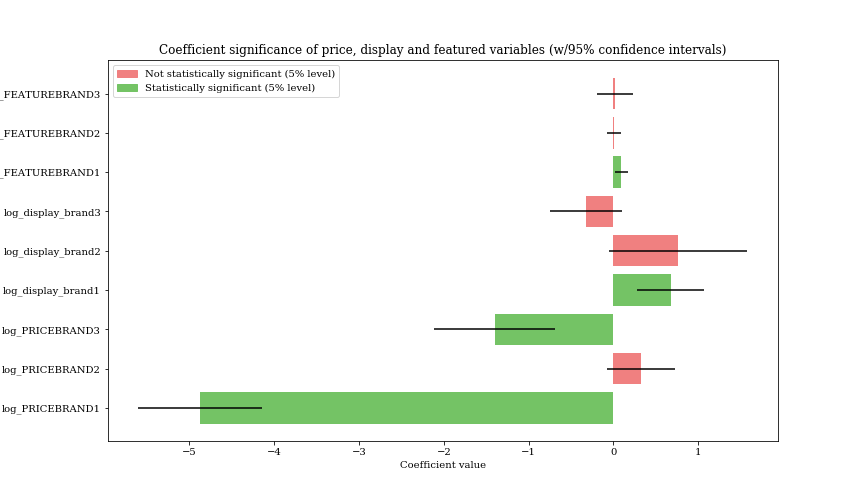
\includegraphics[scale=0.47]{brand1_modelfinal_significance}
  \caption{Brand 1 key model coefficients with confidence intervals }\label{fig:brand1-significance}
\end{figure}

\begin{figure}
  \centering
  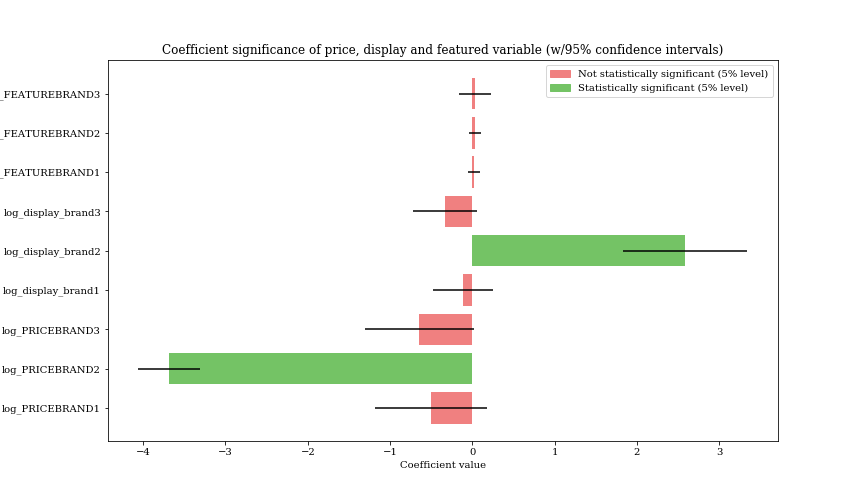
\includegraphics[scale=0.47]{brand2_modelfinal_significance}
  \caption{Brand 2 key model coefficients with confidence intervals }\label{fig:brand2-significance}
\end{figure}

\begin{figure}
  \centering
  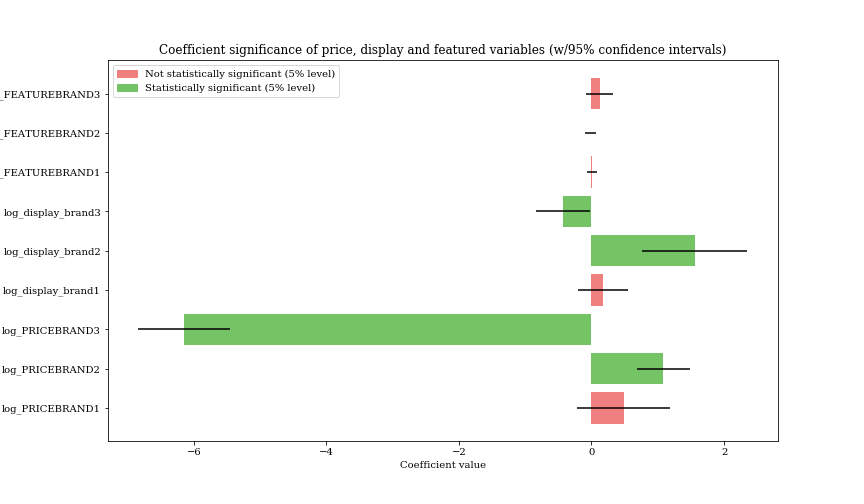
\includegraphics[scale=0.47]{brand3_modelfinal_significance}
  \caption{Brand 3 key model coefficients with confidence intervals }\label{fig:brand3-significance}
\end{figure}

\subsection{Price}

The own brand price elasticities of brand 1, 2 and 3 are -4.874, -3.682, -6.141 respectively. Due to the log-log form of the model, these coefficients can be interpreted as meaning that a decrease in price by 1\% will increase the unit sales by 4.874\%, 3.682\% and 6.141\% for each brand respectively. This suggests that customers of brand 3 are most sensitive to changes in price. The confidence intervals for the own brand price elasticities are small compared to the magnitude of the coefficient which gives confidence of the sign and relative magnitude of these coefficients.

The cross-brand price elasticities are much lower than the own-brand price elasticities. Indicating consumers are less sensitive to competitor pricing and use any price discounts to stock up on their preferred brand of beer (forward purchase effect).


\subsection{Display}

The own brand display coefficients are 0.674, 2.583, -0.429 for each brand respectively. This implies that if the percentage of SKUs on display for each brand is increased by 1\% (note this is not the same as an increase by 1 \textit{percentage point}), then the unit sales for the week are increased by 0.674\% and 2.583\% for brands 1 and 2 whereas the unit sales are decreased by 0.429\% for brand 3. Display promotions are therefore most effective for brand 2 with a significant uplift in sales when a greater percentage of SKUs are on display. Display promotions are less effective for brand 1 and actually detrimental for brand 3. Brand 3 is the least popular of the three brands in terms of unit sales and customers which may be a reason why customers may not respond as well to the promotion.

\subsection{Feature}

The feature variables in the model are binary and therefore their coefficients are interpreted differently to the price and display variables. The effect on unit sales of the \textit{binary\_FEATUREBRAND*} variables is equal to $e^{coefficient}$. The own brand feature coefficients for brand 1, 2 and 3 are 0.094, 0.033, 0.123 respectively. However, only brand 1's coefficient is statistically significant. Therefore, if brand 1 is featured during the week then unit sales are increased by approximately 9.9\% ($e^0.094 = 1.099)$. The lower 95\% confidence interval for this coefficient is greater than 0, therefore it can be concluded that featuring brand 1 has a positive effect on sales.

The own brand coefficients for brand 2 and 3 are not statistically significant but are both positive. This suggests that featuring these brands in the week has a positive impact on sales as well, however, we can not be as confident in the magnitude of the effect. The low confidence in these coefficients may be a result of the fact that in the available data a lower percentage of SKUs were featured for brands 2 and 3 compared to brand 1 (figure \ref{fig:eda-plots}). This information was lost when converting to a binary variable therefore the effect of feature promotions is harder to discern.


\section{Conclusions}

The SCAN*PRO model can be used to estimate unit sales with good accuracy and consistency across different brands of beer (table \ref{tab:val-results}). Seasonality is the largest contributing factor to unit sales, however, price, display and feature promotional activity is also statistically significant. 

Decreasing the price of the beer brand can increase unit sales by between 3.7-6.1\%. Display and feature promotions are not equally effective for all brands. Display advertising works best for brand 2 with an uplift in unit sales of 2.5\% for every percentage point increase in SKUs on display, whereas there is only a minimal effect for brands 1 and 3. Feature advertising has a greater impact on unit sales than display promotions with an uplift of 9.9\% observed for brand 1, however, only brand 1 had a statistically significant coefficient.


\subsection{Management Recommendations}
The following recommendations can be made to the store manager of Dominick's:
\begin{itemize}
    \item Use 'feature' advertising to promote brand 1 preferentially.
    \begin{itemize}
        \item Feature promotions are most effective for brand 1 with a potential uplift of sales by 9.9\% in weeks where brand 1 is featured. Brand 2 and 3 feature promotions are not effective.
    \end{itemize}
    \item Combine display promotions with regular price reductions for brand 2.
    \begin{itemize}
        \item Display advertising is most beneficial for brand 2 with an increase in unit sales of 2.5\% for every percentage point increase in SKUs on display. This should be combined with regular price reductions which could increase sales by a further 3.7\% for every 1\% reduction in price.
    \end{itemize}
    \item Only utilise regular price discounts to promote brand 3
    \begin{itemize}
        \item Brand 3 customers are most price sensitive. Decreasing prices of brand 3 by 1\% can increase unit sales by 6.74\%. Brand 3 is a less popular brand of beer and does not respond well to display or feature advertising. Therefore, regular price discounting will have the greatest effect for increasing unit sales. 
    \end{itemize}
    

\end{itemize}

\subsection{Model Improvements}
While the accuracy and fit of the SCAN*PRO models to the data were reasonably high ($R^2 \approx 0.8$), the model accuracy and $R^2$ could be further improved. During regression modelling it was observed that there were a number of data points in the sample with high leverage which could have materially affected the model coefficients. These points could be removed from fitting the model to improve the confidence in the model coefficients. Secondly, additional features could be added to the model which are correlated to beer sales such as promotional activity of competing alternative products, for example wine or spirits, which may also affect a customer's propensity to buy beer.

\subsection{Future Work}
This analysis focuses on increasing the unit sales of each beer brand. The profit margin for the store was not considered. Further work could aim to use the information about promotions from this analysis to find the optimum promotional allocation to maximise store profits (i.e. balance trade off between reducing retail price to increase unit sales and maintaining a profit margin).

The SCAN*PRO model only addresses the short-term impact of price changes and promotional activity on demand for the product. It would also be useful for the store manager be able to understand the long-term impact of promotional activity on future unit sales due to the forward and delayed purchase effects that promotions have on customer purchasing behaviour. This can be quantified using VAR and IRFS models [REFERENCE] .  


\textbf{Word Count: 2,619}

\bibliographystyle{agsm}
\bibliography{references}




\end{document}
